\section{Resultados y discusión}

\subsection{Análisis Cuantitativo}

\subsubsection{Objetivo:}

Realizamos dos pruebas del tiempo de cómputo necesario para resolver el problema del presente trabajo.
En el primero variamos la cantidad de páginas manteniendo una proporción de los links entre ellas.
En el segundo fijamos la cantidad de páginas y variamos la densidad de la misma.


Nodos:
Ejes: Mantenemos la cantidad de nodos fijos en 1000, iteramos 25 veces desde cantidad de ejes en 8000 aumentando en 8000 en cada iteracion repitiendo el cálculo 5 veces y promediándo el tiempo reportado.


\subsubsection{Hipótesis:}

asd

\subsubsection{Resultado y Análisis: }

Nodos:

\begin{figure}[h]
   \begin{center}
     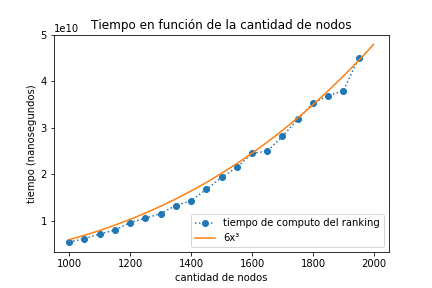
\includegraphics{img/tiempo_nodos_prop.png} 
  \end{center}
\caption{Tiempo en función de la cantidad de nodos} \label{fig:exp1-nodos}
\end{figure}


Ejes:

\begin{figure}[h]
   \begin{center}
     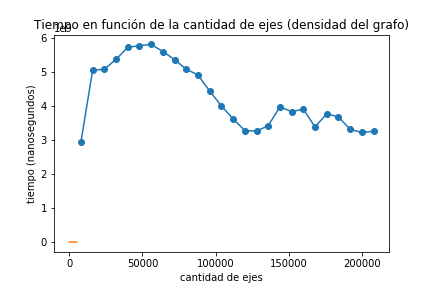
\includegraphics{img/tiempo_ejes.png} 
  \end{center}
\caption{Tiempo en función de la cantidad de ejes} \label{fig:exp1-ejes}
\end{figure}

P:


\begin{figure}[h]
   \begin{center}
     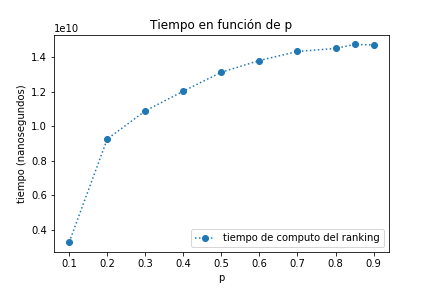
\includegraphics{img/tiempo_p.png} 
  \end{center}
\caption{Tiempo en función de la cantidad de nodos} \label{fig:exp1-p}
\end{figure}


\subsection{Análisis Cualitativo}

\subsubsection{Objetivo:}

En la presente sección se busca analizar la calidad de los rankings calculados por el método de Page Rank, evaluarlo según el contexto en el que se lo aplique y relacionándolo con la estructura del grafo subyacente a la red de páginas web a las que deseamos asignarles algún valor de preferencia.

\subsubsection{Hipótesis:}

asd

\subsubsection{Resultado y Análisis: }

asd

\begin{figure}[h]
   \begin{center}
     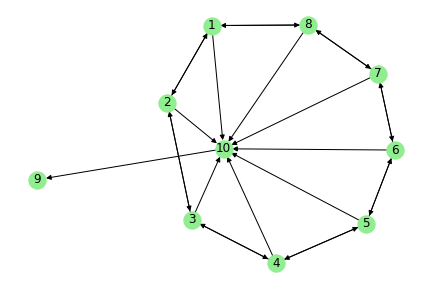
\includegraphics{img/prueba-circular.png} 
  \end{center}
\caption{Redes utilizadas como datos de entrada para el experimento.} \label{fig:exp3-webs}
\end{figure}

\begin{figure}[h]
   \begin{center}
     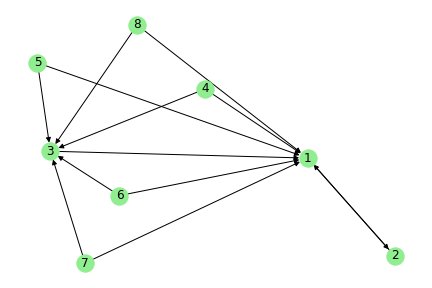
\includegraphics{img/prueba_grafo_2.png} 
  \end{center}
\caption{Redes utilizadas como datos de entrada para el experimento.} \label{fig:exp3-webs}
\end{figure}

\begin{figure}[h]
   \begin{center}
     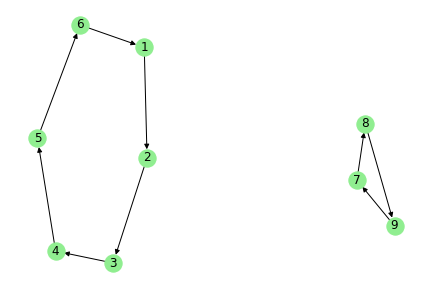
\includegraphics{img/prueba_3_no_conexa.png} 
  \end{center}
\caption{Redes utilizadas como datos de entrada para el experimento.} \label{fig:exp3-webs}
\end{figure}